%! Author = fusel
%! Date = 24.07.21

% Preamble
\documentclass[final]{fhnwreport}
% Packages
\usepackage{amsmath}
\usepackage{lipsum}
\usepackage[german]{babel}
\usepackage[style=ieee,urldate=comp,backend=biber]{biblatex}
\usepackage{listings}
\usepackage{xcolor}
\usepackage{dirtree}
\usepackage{textcomp}
\addbibresource{main.bib}

% Custom JS Listing support
\definecolor{mygreen}{rgb}{0,0.6,0}
\definecolor{mygray}{rgb}{0.5,0.5,0.5}
\definecolor{mymauve}{rgb}{0.58,0,0.82}
%Customize a bit the look
\lstset{ %
    backgroundcolor=\color{white}, % choose the background color; you must add \usepackage{color} or \usepackage{xcolor}
    basicstyle=\footnotesize, % the size of the fonts that are used for the code
    breakatwhitespace=false, % sets if automatic breaks should only happen at whitespace
    breaklines=true, % sets automatic line breaking
    captionpos=b, % sets the caption-position to bottom
    commentstyle=\color{mygreen}, % comment style
    deletekeywords={...}, % if you want to delete keywords from the given language
    escapeinside={\%*}{*)}, % if you want to add LaTeX within your code
    extendedchars=true, % lets you use non-ASCII characters; for 8-bits encodings only, does not work with UTF-8
    frame=single, % adds a frame around the code
    keepspaces=true, % keeps spaces in text, useful for keeping indentation of code (possibly needs columns=flexible)
    keywordstyle=\color{blue}, % keyword style
% language=Octave, % the language of the code
    morekeywords={*,...}, % if you want to add more keywords to the set
    numbers=left, % where to put the line-numbers; possible values are (none, left, right)
    numbersep=5pt, % how far the line-numbers are from the code
    numberstyle=\tiny\color{mygray}, % the style that is used for the line-numbers
    rulecolor=\color{black}, % if not set, the frame-color may be changed on line-breaks within not-black text (e.g. comments (green here))
    showspaces=false, % show spaces everywhere adding particular underscores; it overrides 'showstringspaces'
    showstringspaces=false, % underline spaces within strings only
    showtabs=false, % show tabs within strings adding particular underscores
    stepnumber=1, % the step between two line-numbers. If it's 1, each line will be numbered
    stringstyle=\color{mymauve}, % string literal style
    tabsize=2, % sets default tabsize to 2 spaces
    title=\lstname % show the filename of files included with \lstinputlisting; also try caption instead of title
}
%END of listing package%

\definecolor{darkgray}{rgb}{.4,.4,.4}
\definecolor{purple}{rgb}{0.65, 0.12, 0.82}

%define Javascript language
\lstdefinelanguage{JavaScript}{
    keywords={typeof, new, true, false, catch, function, return, null, catch, switch, const, let, var, if, in, while, do, else, case, break},
    keywordstyle=\color{blue}\bfseries,
    ndkeywords={class, export, boolean, throw, implements, import, this},
    ndkeywordstyle=\color{darkgray}\bfseries,
    identifierstyle=\color{black},
    sensitive=false,
    comment=[l]{//},
    morecomment=[s]{/*}{*/},
    commentstyle=\color{purple}\ttfamily,
    stringstyle=\color{red}\ttfamily,
    morestring=[b]',
    morestring=[b]"
}

\lstset{
    language=JavaScript,
    extendedchars=true,
    basicstyle=\footnotesize\ttfamily,
    showstringspaces=false,
    showspaces=false,
    numbers=left,
    numberstyle=\footnotesize,
    numbersep=9pt,
    tabsize=2,
    breaklines=true,
    showtabs=false,
    captionpos=b
}



\title{Cloudbasiertes Praxisrufsystem}  %Project Title
\author{IP 5}                      %Document Type => Technical Report, ...

\begin{document}
    \maketitle
    \begin{figure}[h]\label{fig:title}
        
\includegraphics[width=\linewidth]{graphics/wip}\caption[Titlebild]{Titlebild}
    \end{figure}

    \begin{center}
        \renewcommand\arraystretch{2}
        \begin{tabular}{l l}
            Studenten & Joshua Villing, Kevin Zellweger\\
            Fachbetreuer & Daniel Jossen\\
            Auftraggeberin & Daniel Jossen\\
            Studiengang & Informatik\\
            Hochschule & Hochschule für Technik
        \end{tabular}
    \end{center}

    \clearpage


%%---ABSTRACT----------------------------------------------------------------------------
    \pagenumbering{Roman}
    \begin{abstract}
Das Abstract ist eine Art Zusammenfassung des ganzen Dokuments. Es gibt einen Einblick in die Aufgabenstellung, wie diese umgesetzt wurde und welches Ergebnis erreicht wurde. Aus diesem Grund wird das Abstract immer ganz am Schluss der Arbeit verfasst. Es besteht aus einem zusammengehörenden Absatz und umfasst ungefähr 10 bis 20 Zeilen.
Formeln, Referenzen oder andere Unterbrechungen haben im Text nichts zu suchen.
Direkt unter dem Abstract folgt eine Liste von drei bis vier Stichworten/Keywords. Diese werden in alphabetischer Reihenfolge aufgelistet und beschreiben das Themengebiet der Arbeit.

\vspace{2ex}

\textbf{Keywords: Anleitung, LaTeX, Thesis, Vorlage}

\vspace{2ex}

\textbf{Management Summary} siehe PF-IK.

\end{abstract}	

\clearpage

\section*{Vorwort}

\lipsum[1-2]

Fakultativ, siehe PF-IK (URL)


%%---TABLE OF CONTENTS-------------------------------------------------------------------
    \setcounter{tocdepth}{2}
    \tableofcontents
    \clearpage

%%---TEXT--------------------------------------------------------------------------------
    \pagenumbering{arabic}
    \section{Einleitung}

\lipsum[3-4]

Einleitungsbeispiele siehe PF-IK (URL)
    \section{Vorgehensweise}

\subsection{Stakeholder}
\begin{itemize}
    \item Daniel Jossen
    \item Kevin Zellweger
    \item Joshua Villing
\end{itemize}
\subsection{Kommunikation}
\begin{itemize}
    \item Teams
    \item OneNote
    \item Github
\end{itemize}
\subsection{Projektplan}
    \section{Anforderungen}

\subsection{Fachlich}
\subsection{Technisch}

    \section{Evaluation Technologien}

\subsection{Mobile Client}



\url{https://kotlinlang.org/lp/mobile/}
	

    +Jet Brains Infrastructure 
    +We like Kotlin 

    -IoS Env. Needed to develop for Apple 
    -Still has to develop separate API und UI Modules for Platforms 

\url{https://web.dev/progressive-web-apps/ }
	
    +No need of Native Codebase
    +Perfect for Android 
    -Eventually drawbacks because no entire API Access 
    -PWAs on IOS suck

\url{https://cordova.apache.org/} 
	

    + Popular Framework 
    + Tons of plugins to access apis 

    -Still need to have a Mac for IoS development  
    -Not a truly native app -> API Issues
 

\url{https://nativescript.org/ }

    +Provides a Workaround for nasty X-tools 
    +Claims to be truly Native 
    -Do we really trust it? (sorta new and passion project of a few people) 

 
 \url{https://flutter.dev}

    -Why do you hate me?


"Simply Write Everything twice"

    +Would definitely work

    -Do most things twice
    -We don't have time for that
    -Kunde wünscht ausdrücklich nur eine Codebasis für beide Clients.
	

  

\url{https://stackshare.io/stackups/apache-cordova-vs-nativescript 

\url{https://nativescript.org/blog/build-nativescript-apps-remotely-from-windows-or-linux/ }

\subsection{Cloud Service}

    \url{https://aws.amazon.com/  }

    \url{https://spring.io/projects/spring-boot } 

    Konfig der Clients könnte sich als No-SQL anbieten.   

    Config muss nur gelesen und an den Client geschickt oder abgespeichert werden  

    \url{https://www.mongodb.com/}  

  

\subsection{Betrieb und Platform}

AWS ist MUSS
    \section{Konzept}\label{sec:konzept}
\subsection{Systemarchitektur}\label{subsec:systemarchitektur}
\subsubsection*{Überblick}

Für das Cloudbasierte Praxisruf System sehen wir fünf Komponenten vor:

\begin{itemize}
    \item Messaging Service
    \item Cloud Service
    \item Mobile Client
    \item Admin UI
    \item VOIP Mediator
\end{itemize}


\begin{figure}
    \centering
    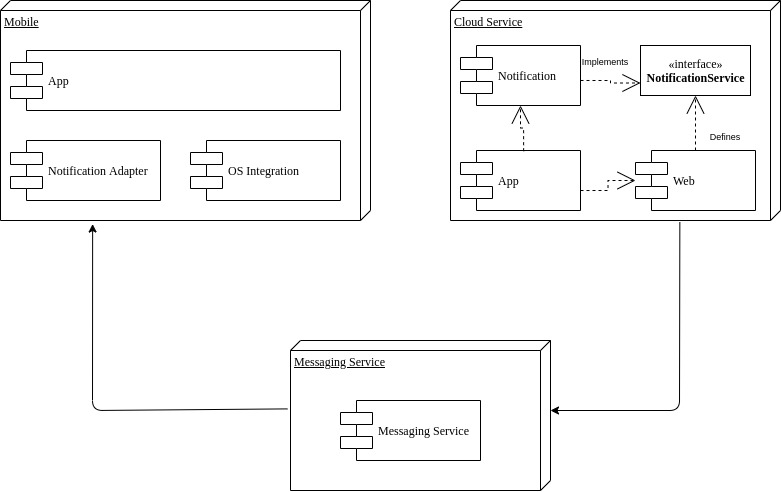
\includegraphics[width=\linewidth]{graphics/IP5_POC_Cloud_Architecture}\label{fig:architecure}
\end{figure}


\subsubsection*{Mobile Client}

\begin{itemize}
    \item Der Mobile Client implementiert die Anbindung an den Messaging Service.
    \item Als Reaktion auf eine Notification wird eine Rückmeldung im UI angezeigt.
    \item Als Reaktion auf eine Notification wird eine OS Push Notifikation gesendet.
    Das UI bietet einen Button der eine Anfrage an die REST Schnittstelle im Cloud Service sendet.
\end{itemize}


\subsubsection*{Cloud Service}

\begin{itemize}
    \item Responsibilities (Notification and Configuration)
    \item Microservice Granularity
\end{itemize}


\subsubsection*{Messaging Service}

\begin{itemize}
    \item Dies wird ein externer Service den wir in die Applikationen einbinden. Standard hierfür ist Firebase Notifications.
    \item Der Messaging Service nimmt Notifikationen vom Cloud Service entgegen und gibt diese an den Mobile Client wieder.
    \item Dafür müssen auf beiden Seiten Komponenten eingebaut werden, die mit dem Messaging Service kommunizieren.
\end{itemize}

\clearpage

\subsection{Mobile Client}\label{subsec:mobile-client}

\subsubsection{Framework Grundlagen}
NativeScript bietet eine Abstraktion zu den nativen Plattformen Android und IOS.
Die jeweilige NativeScript Runtime erlaubt es in Javascript (oder einem entsprechenden Application Framework) Code zu schreiben,
welcher direkt für die entsprechende native Umgebung kompiliert wird~\cite{ns-core-overview}.
\begin{figure}[h]
    \centering
    \label{fig:howNSWorks}
    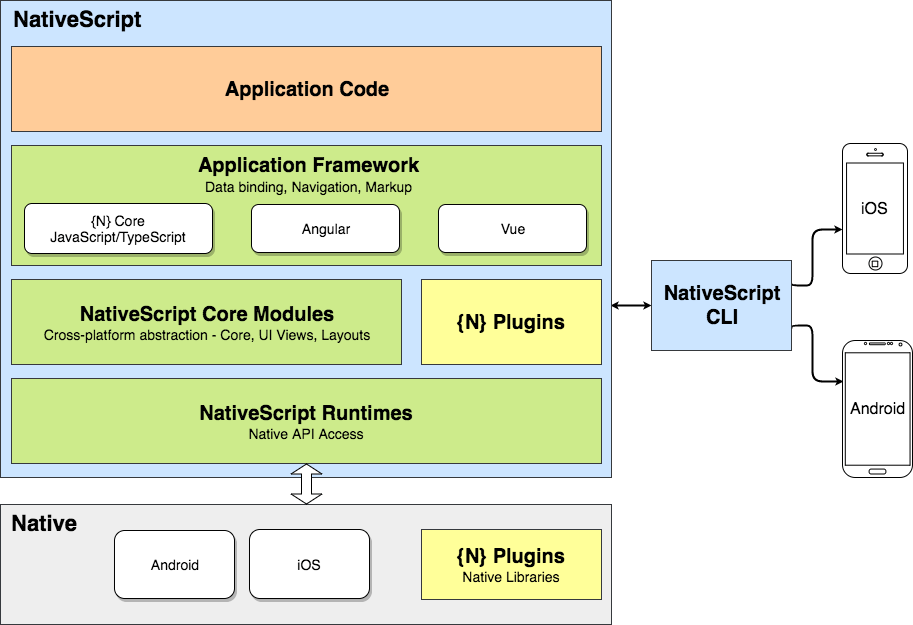
\includegraphics[width=0.7\textwidth]{graphics/ns-common}\caption[NativeScript-Overview]{NativeScript-Overview}\textcopyright OpenJS Foundation
\end{figure}


Die Runtime agiert als Proxy zwischen Javascript und dem jeweiligen Ökosystem.
Im Falle von IOS bedeutet dies u.A. das für alle Objective-C types ein JavaScript Prototype angeboten wird.
Dies ermöglicht es direkt mit nativen Objekten zu interagieren.
Im Umkehrschluss findet eine Typenkonversion via Marshalling Service statt\cite{ns-ios-runtime}.

\subsubsection{Architektur}
Wir verwenden NativeScript Core als Framework des Mobile-Clients.
In Kapitel \emph{\nameref{subsec:mobile-client-eval}} gehen wir auf die weiteren verfügbaren Frameworks ein und erläutern, weshalb wir uns gegen sie entschieden haben.

Die Client-Applikation ist in Module unterteilt.
Ein Modul wird aus folgenden Komponenten definiert:
\begin{itemize}
    \item UI-Markup: Statische Darstellung in XML
    \item Backend: Verhalten und Dynamisierung in Javascript
    \item Styling: Layout und Styles in CSS
\end{itemize}

Ein minimales Modul kann alleine aus einer XML-Datei bestehen.
Die optionalen Javascript und CSS Dateien müssen denselben Namen haben wie die XML Datei, um vom Framework korrekt verknüpft zu werden.
Dateien mit anderen Namen werden grundsätzlich vom Framework ignoriert.
Natürlich steht es Frei dennoch solche Dateien anzulegen und deren Funktionen zu verwenden z.~B. als \emph{\nameref{subsubsec:services}} oder als \emph{\nameref{subsubsec:code-behind-komponenten}}.

\subsubsection*{Page Module}

\lstinputlisting[caption=home-model.js,language=JavaScript,label={lst:home-model.js}]{listings/home-model.js}
\lstinputlisting[caption=home-page.js,language=JavaScript,label={lst:home-page.js}]{listings/home-page.js}
\lstinputlisting[caption=home-page.xml,language=XML,label={lst:home-page.xml}]{listings/home-page.xml}


\subsubsection*{Code-Behind Komponenten}\label{subsubsec:code-behind-komponenten}
\subsubsection*{Services}\label{subsubsec:services}



\clearpage

\subsubsection{User Interface}
\begin{figure}[h]
    \centering
    \begin{minipage}[b]{0.4\textwidth}
        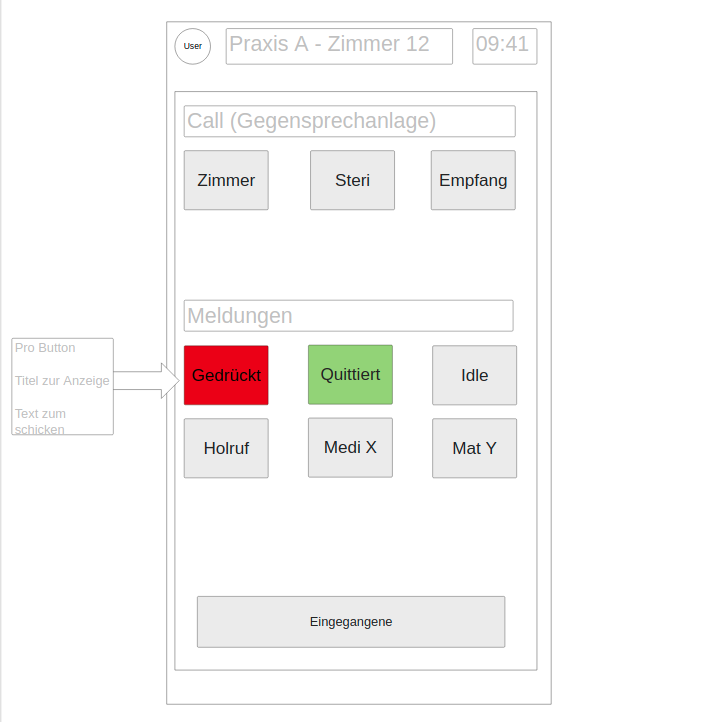
\includegraphics[width=\textwidth]{graphics/homescreen-mockup}
        \caption{HomeScreen Mockup}
    \end{minipage}
    \hfill
    \begin{minipage}[b]{0.4\textwidth}
        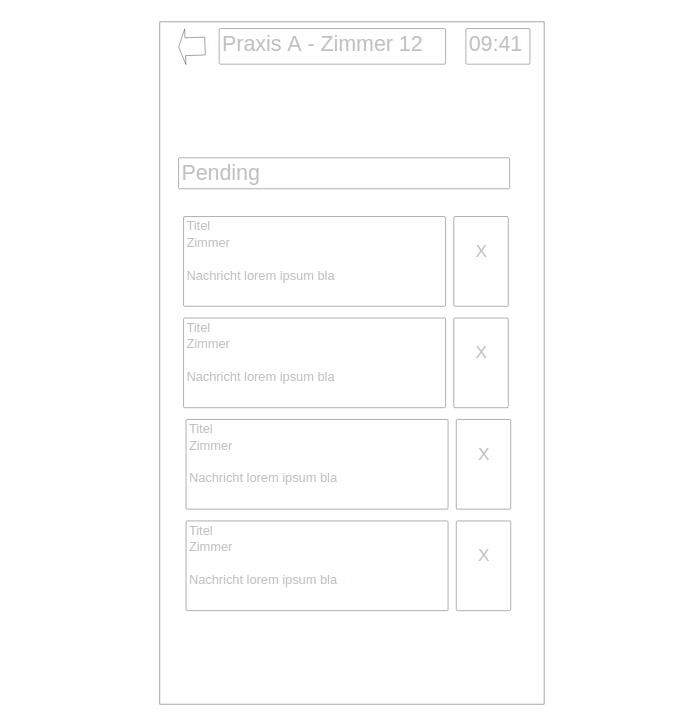
\includegraphics[width=\textwidth]{graphics/mockup-received}
        \caption{Inbox Mockup}
    \end{minipage}\label{fig:MobileClient-Mocks}
\end{figure}


\clearpage

\subsection{Cloud Service}\label{subsec:cloud-service}

\subsubsection{Architektur}

\subsubsection{Domänenmodell}

\subsubsection{Laufzeitmodell}

\clearpage

\subsection{Admin UI}\label{subsec:admin-ui}

\clearpage

\subsection{Proof Of Concept}\label{subsec:proof-of-concept}
\subsubsection*{Anforderungen}
\begin{itemize}
    \item Als \textless Sender Rolle\textgreater möchte ich Notifikationen versenden können.
    \item Als \textless Empfänger Rolle\textgreater möchte ich Notifikationen in der Applikation sehen, wenn die Applikation geöffnet ist.
    \item Als \textless Empfänger Rolle\textgreater möchte ich Notifikationen über das OS erhalten, wenn die Applikation minimiert ist.
\end{itemize}
\subsubsection*{Restriktionen}
\begin{itemize}
    \item Nur 1 Client.
    \item Nur 1 fixe Notifikation. Keine Types.
    \item Notifikation wird vom Client gesendet und vom selben Client empfangen.
    \item Keine Authentication oder Authorization.
\end{itemize}

    \section{Umsetzung}\label{sec:umsetzung}

\subsection{Resultate}

Das Praxisrufsystem wurde wie im Kapitel 5 - Konzept beschrieben umgesetzt.
Es wurden die drei Komponenten Mobile Client, Cloud Service und Admin UI implementiert.
Über den angebundenen Messaging Service Firebase Messaging ist es möglich, Benachrichtigungen zwischen Mobile Clients zu versenden.
Cloud Service und Admin UI ermöglichen es dabei die Benachrichtigungen die Versendet werden können und welcher Client welche Benachrichtungen erhalten soll zu konfigurieren.
Weiter wurde mit Amazon Web Services (AWS) eine CI/CD Umgebung aufgebaut, die es erlaubt Cloud Service und das Admin UI zu betreiben und testen.
Diese Umgebung wird dem Kunden als Template dienen, wie er das Praxisrufsystem in der Praxis betreiben kann\footnote{Siehe Anhang Betriebshandbuch}.

Im Rahmen des Projektes wurden damit die Milestones M01 bis M06\footnote{Siehe Kapitel 2.2} erreicht.
Umgesetzt wurden die Milestones mit den folgenden User Stories inklusive aller dazu definierten Features und Szenarien\footnote{Siehe Kapitel 3}:

\begin{itemize}
    \item U01 - Benachrichtigung versenden
    \item U02 - Benachrichtigungen empfangen
    \item U03 - Nur relevante Benachrichtigungen empfangen
    \item U04 - Auf Benachrichtigungen aufmerksam machen
    \item U05 - Verpasste Benachrichtigungen anzeigen
    \item U06 - Fehler beim Versenden von Benachrichtigungen anzeigen
    \item U07 - Konfiguration auf Mobile Client auswählen
    \item U12 - Mehrere Mobile Clients konfigurieren
    \item U13 - Individuelle Konfiguration pro Mobile Client
    \item U14 - Zentrale Konfigurationsverwaltung
    \item T01 - Mobile Client unterstützt IPads
    \item T02 - Mobile Client unterstützt Android Tablets
    \item T03 - Geteilte Code Basis für Android and IOS
    \item T04 - Betrieb mit AWS
\end{itemize}

Die Milestones M06 bis M10 konnten im Rahmen dieses Projektes nicht umgesetzt werden.
Damit sind folgende User Stories ausserhalb des Projektrahmens gefallen:

\begin{itemize}
    \item U08 - Physicher Knopf am Behandlungsstuhl
    \item U09 - Text To Speech für Benachrichtigungen
    \item U10 - Direkte Unterhaltungen zwischen Mobile Clients
    \item U11 - Gruppenunterhaltungen zwischen Mobile Clients
    \item U15 - Konfiguration von direkten Anrufen
    \item U16 - Konfiguration von Gruppenanrufen
\end{itemize}

\clearpage
\begin{itemize}
    \item Die Gegensprechanlage ist komplett Weggefallen.
    \subitem Grundsätzlich Stünde eine Lib. für IOS in NS zur Verfügung. Der Android Teil ist da noch "TODO"
    \item Die Rückfärbung der Buttons auf Grün ist weggefallen da der Handshake so nicht implmentiert wurde.
\end{itemize}

\clearpage
\subsubsection{Mobile Client}\label{subsec:mobile-client-realisation}

Dieses Kapitel zeigt die umgesetzten Ansichten des Mobile Clients.
Eine detaillierte Beschreibung, wie der Mobile Client bedient werden kann, befindet sich im Anhang der Projektdokumentation.

\begin{figure}[h]
    \centering
    \begin{minipage}[b]{0.4\textwidth}
        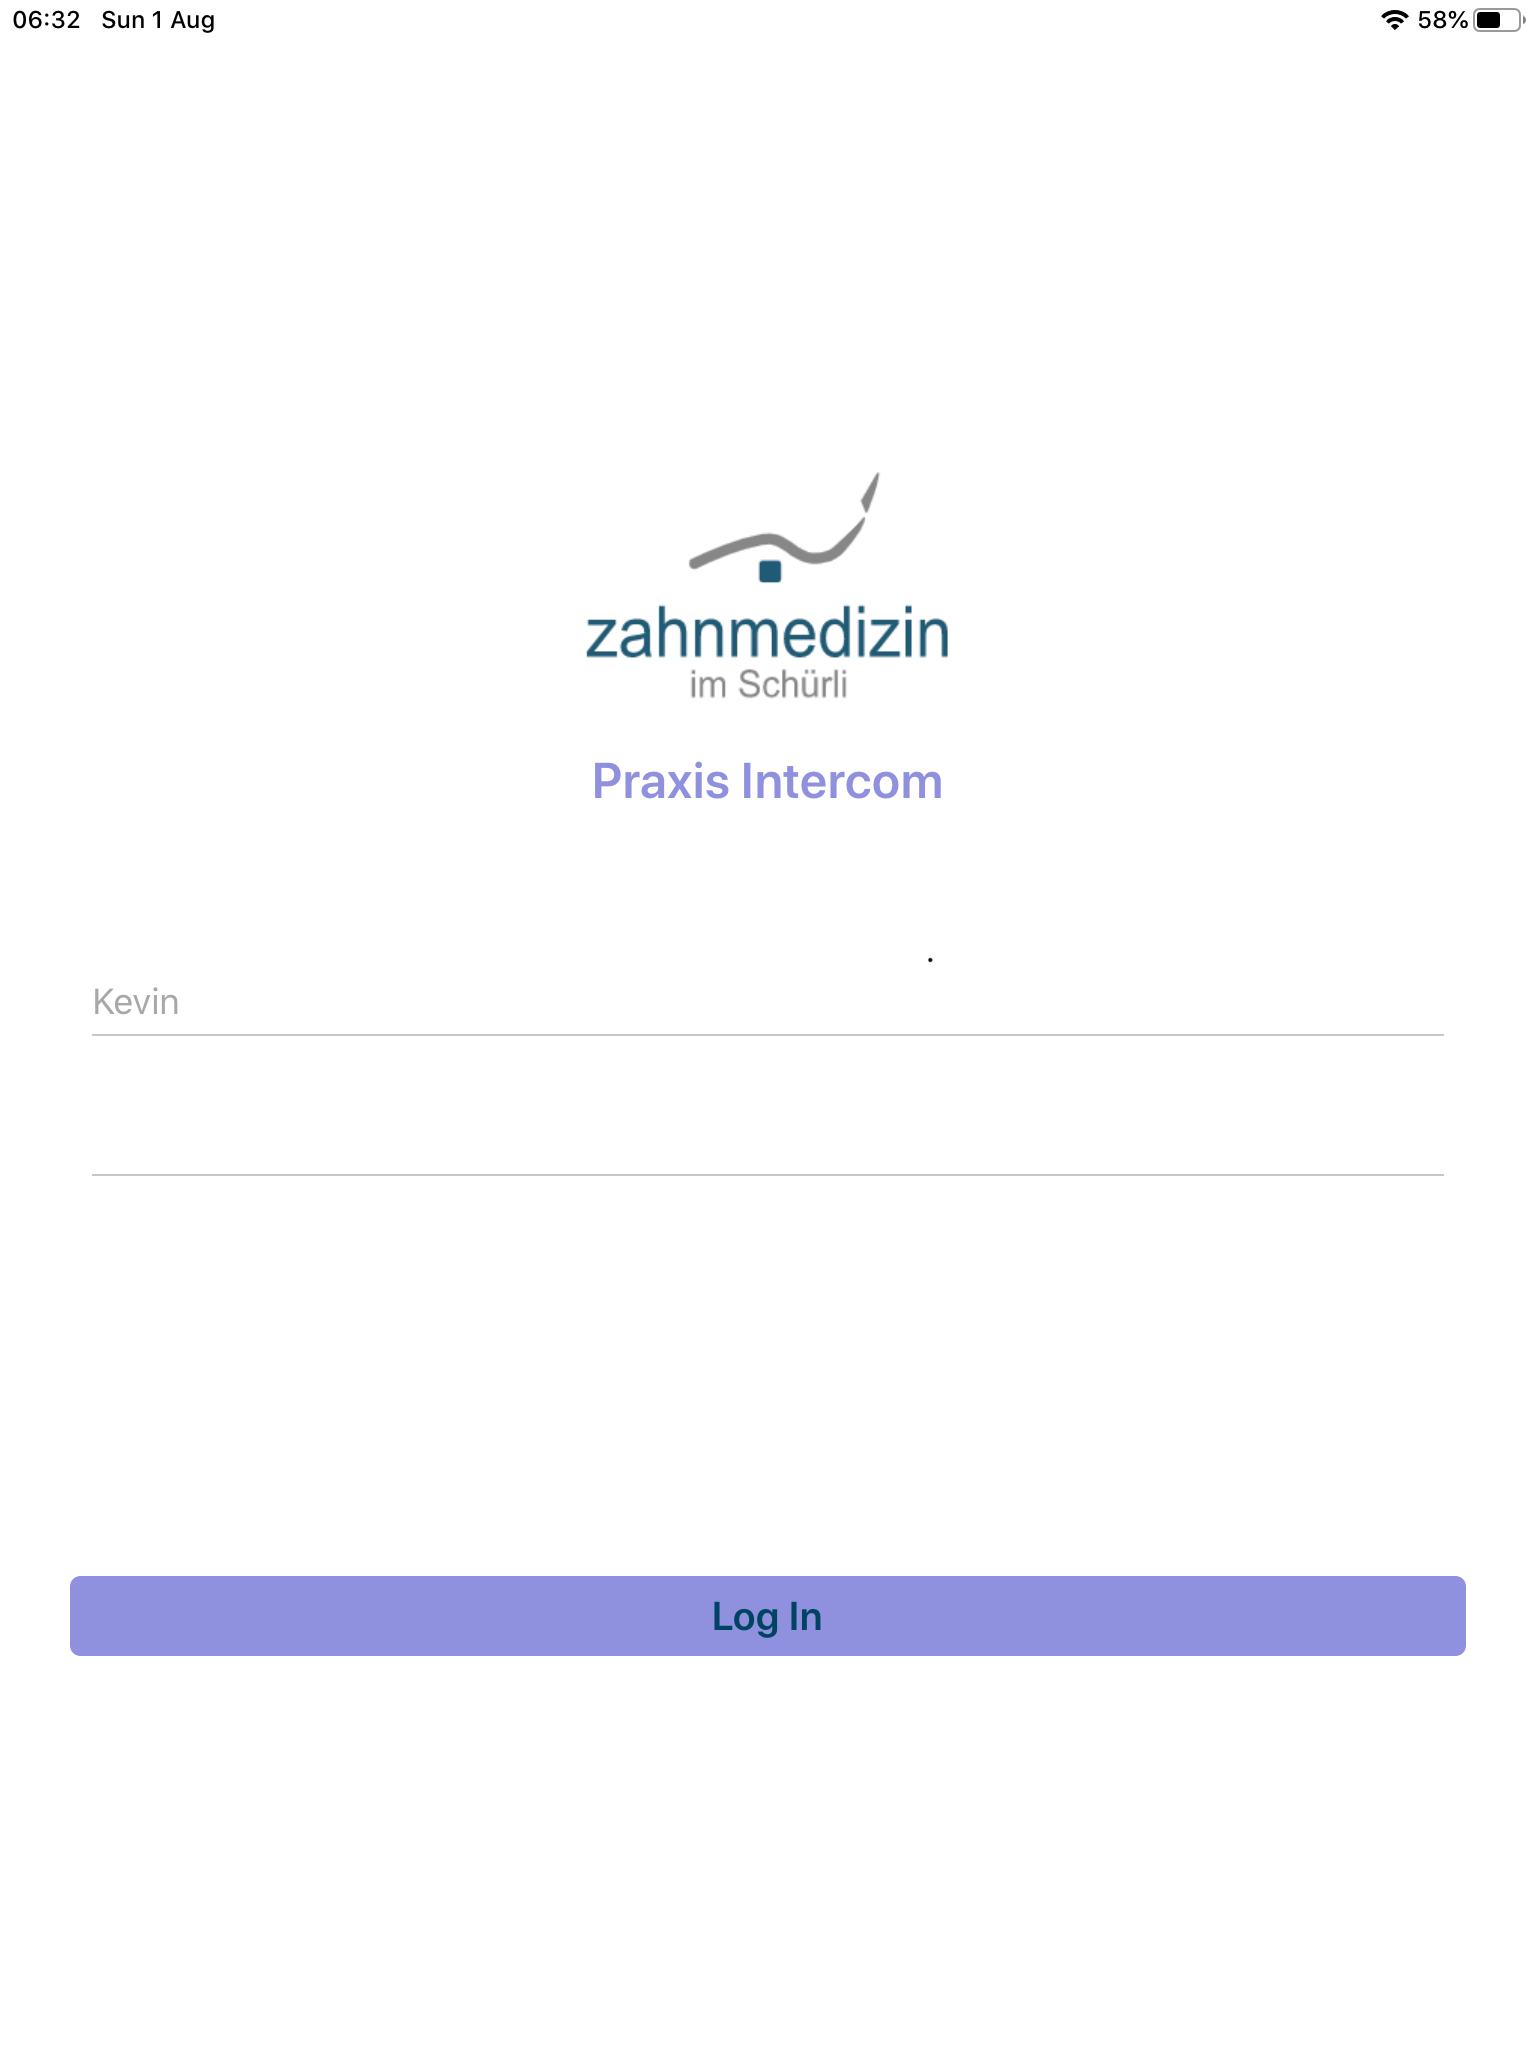
\includegraphics[width=\textwidth]{graphics/screenshot-login}
        \caption{Login}
    \end{minipage}
    \hfill
    \begin{minipage}[b]{0.4\textwidth}
        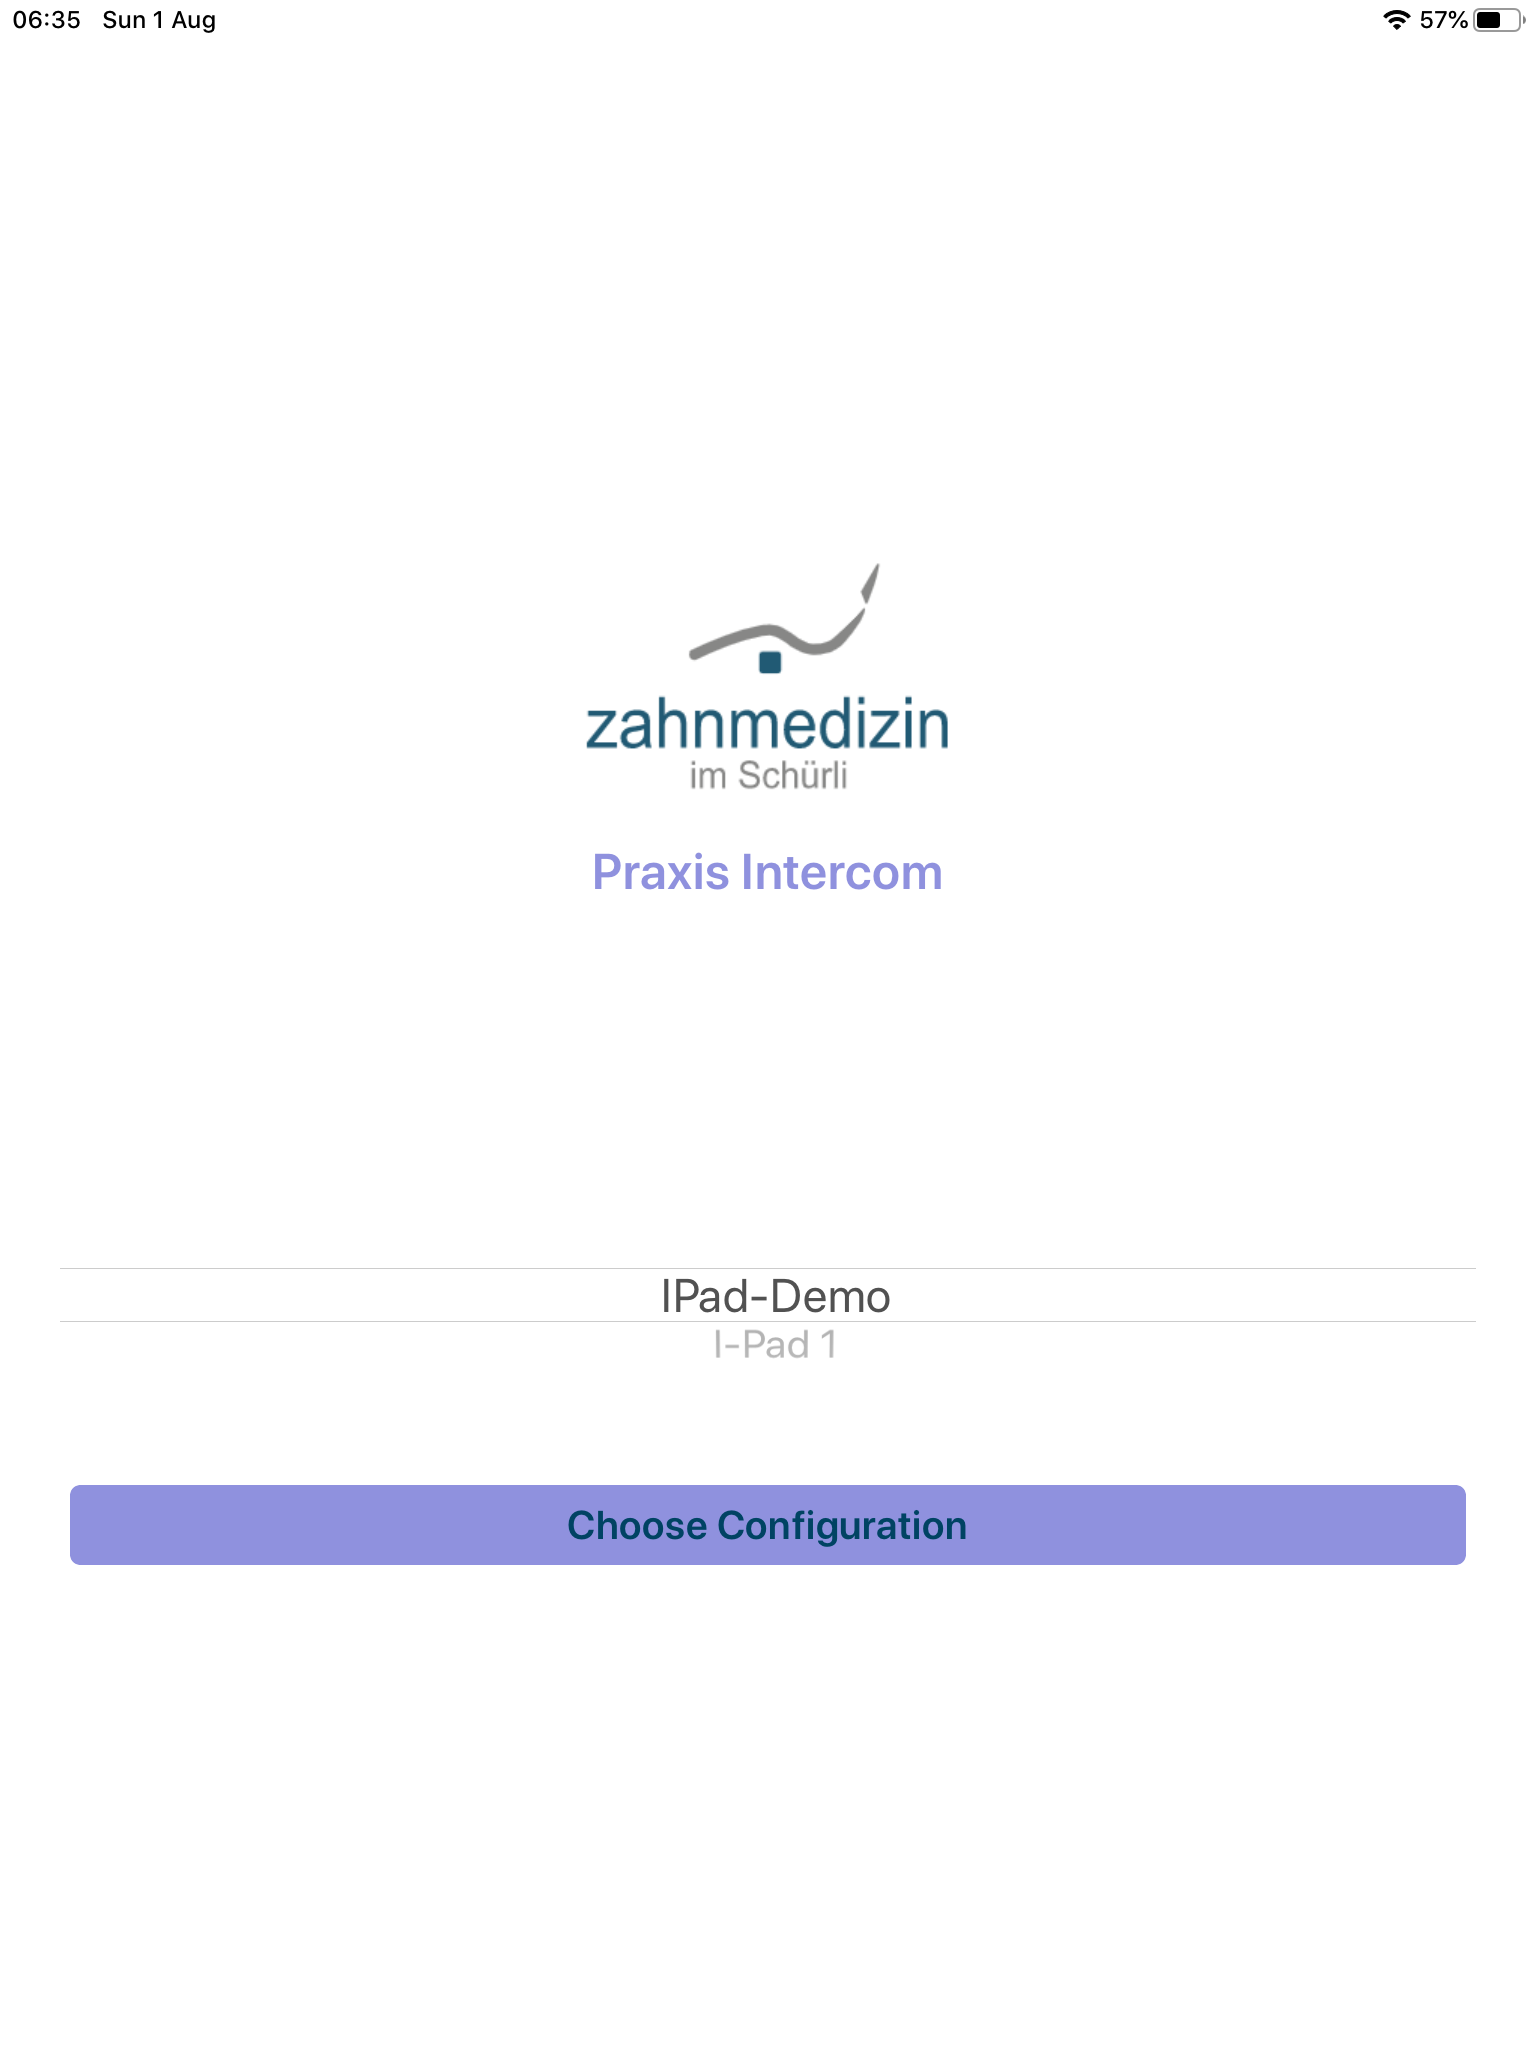
\includegraphics[width=\textwidth]{graphics/screenshots/mobileclient/screenshot-select-config}
        \caption{Konfiguration}
    \end{minipage}
    \label{fig:MobileClient-Screens1}
\end{figure}

\clearpage

Dieses Kapitel zeigt die umgesetzten Ansichten des Admin UIs.
Eine detaillierte Beschreibung, wie der Mobile Client bedient werden kann, befindet sich im Anhang der Projektdokumentation.

\begin{figure}[h]
    \centering
    \begin{minipage}[b]{0.4\textwidth}
        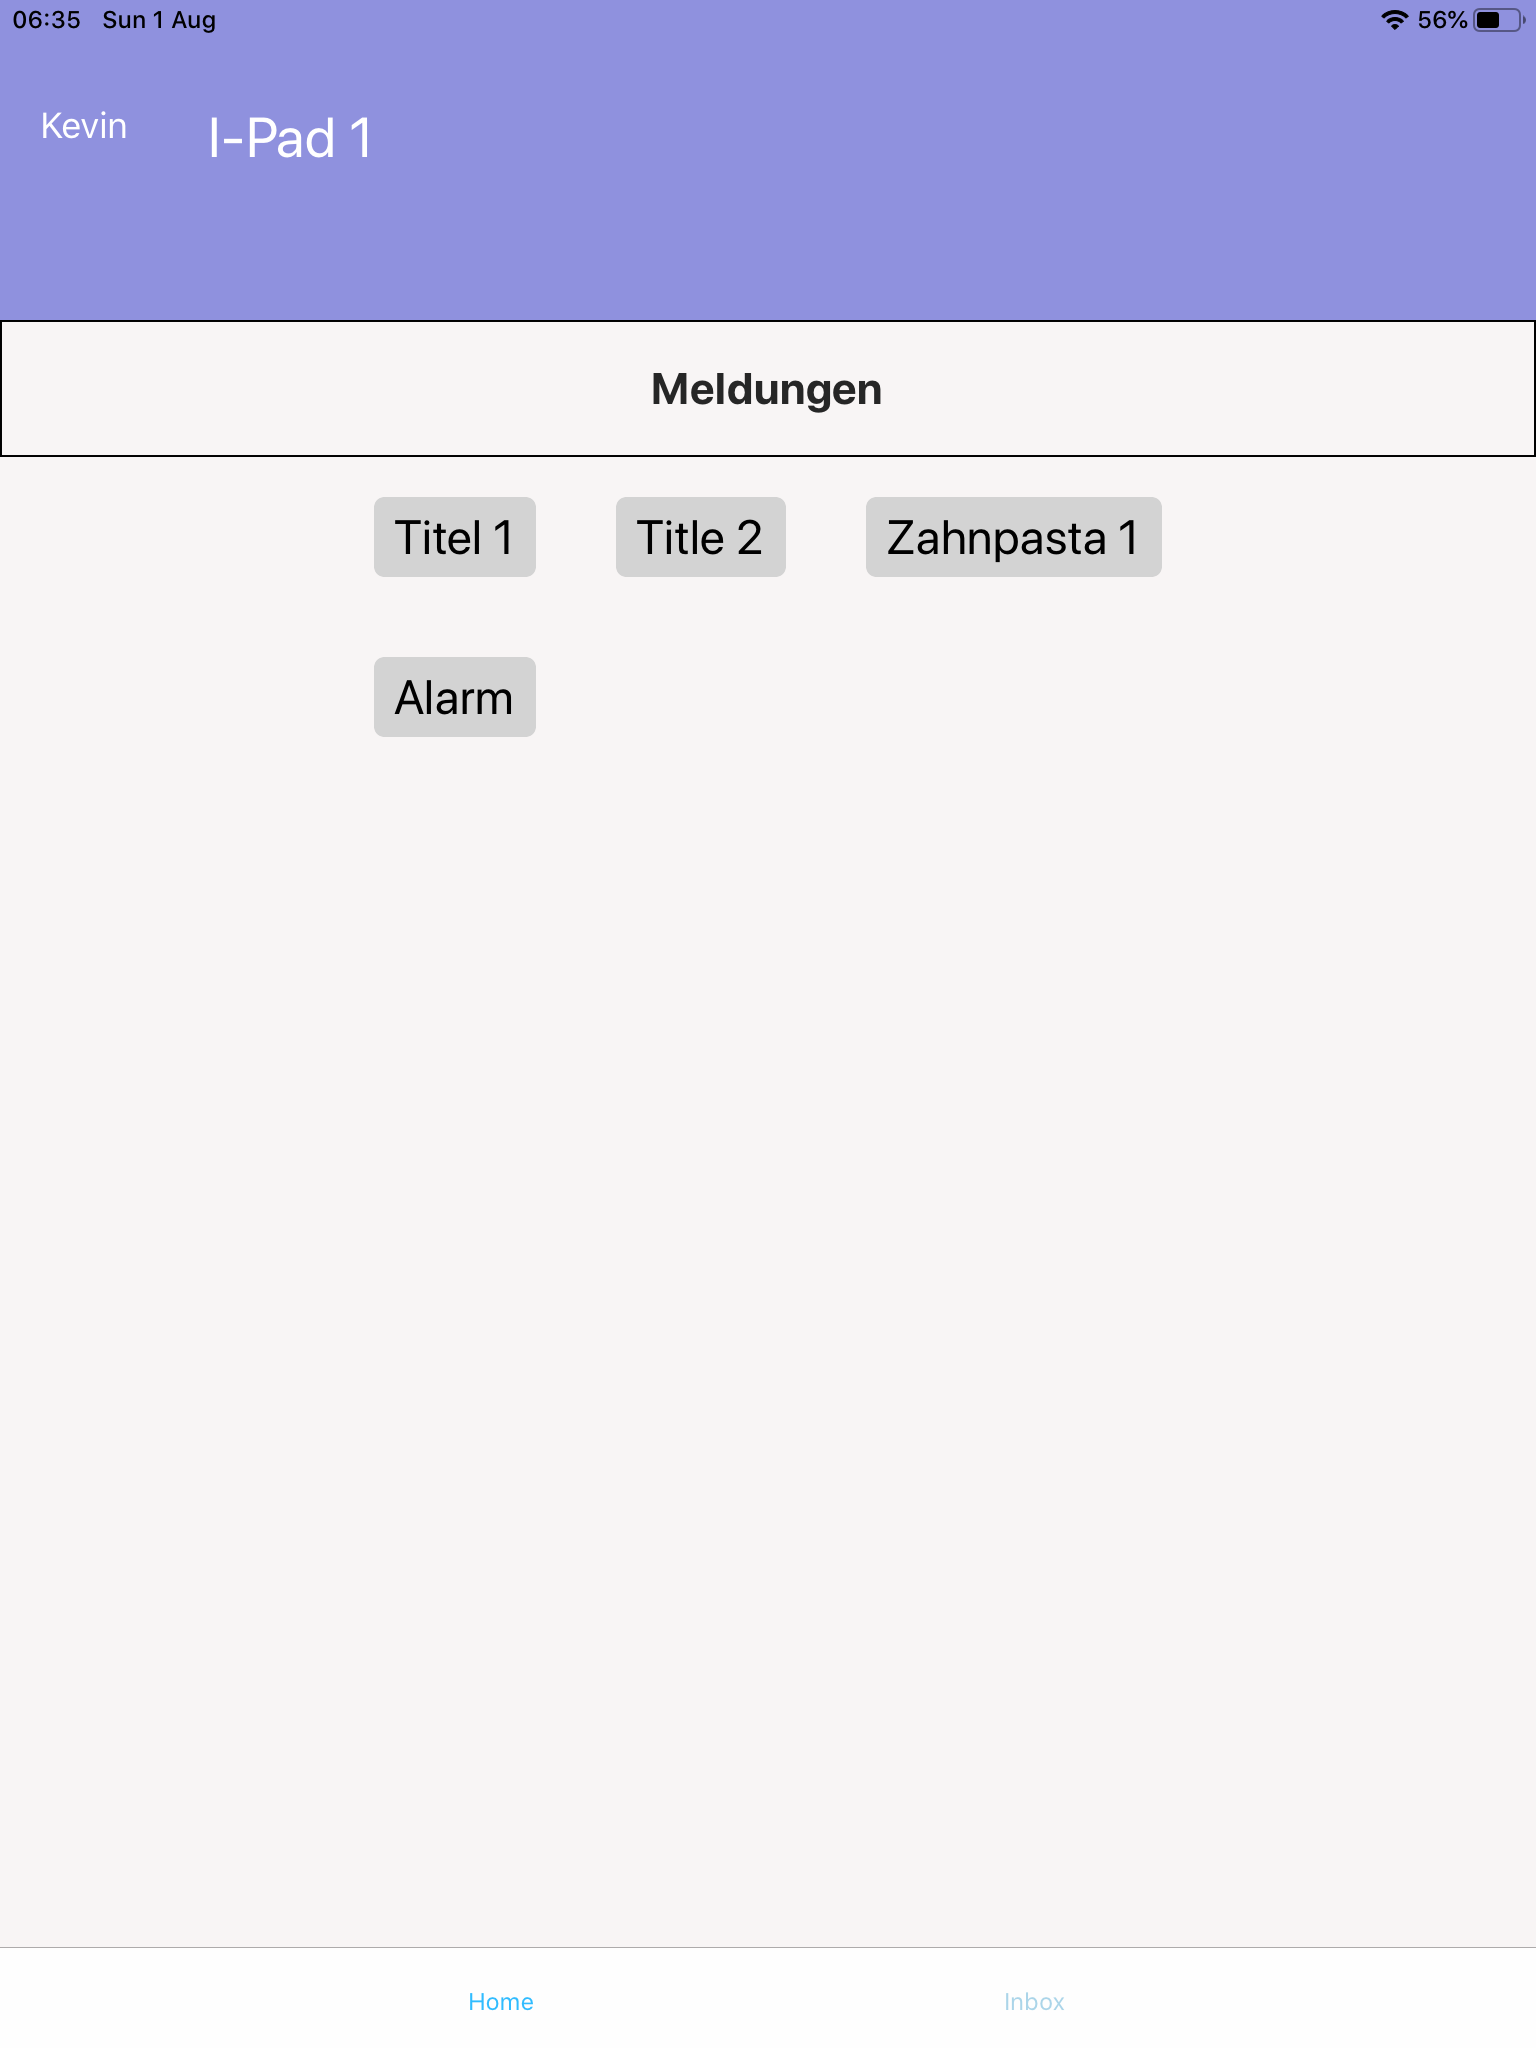
\includegraphics[width=\textwidth]{graphics/screenshots/mobileclient/screenshot-homescreen}
        \caption{Home}
    \end{minipage}
    \hfill
    \begin{minipage}[b]{0.4\textwidth}
        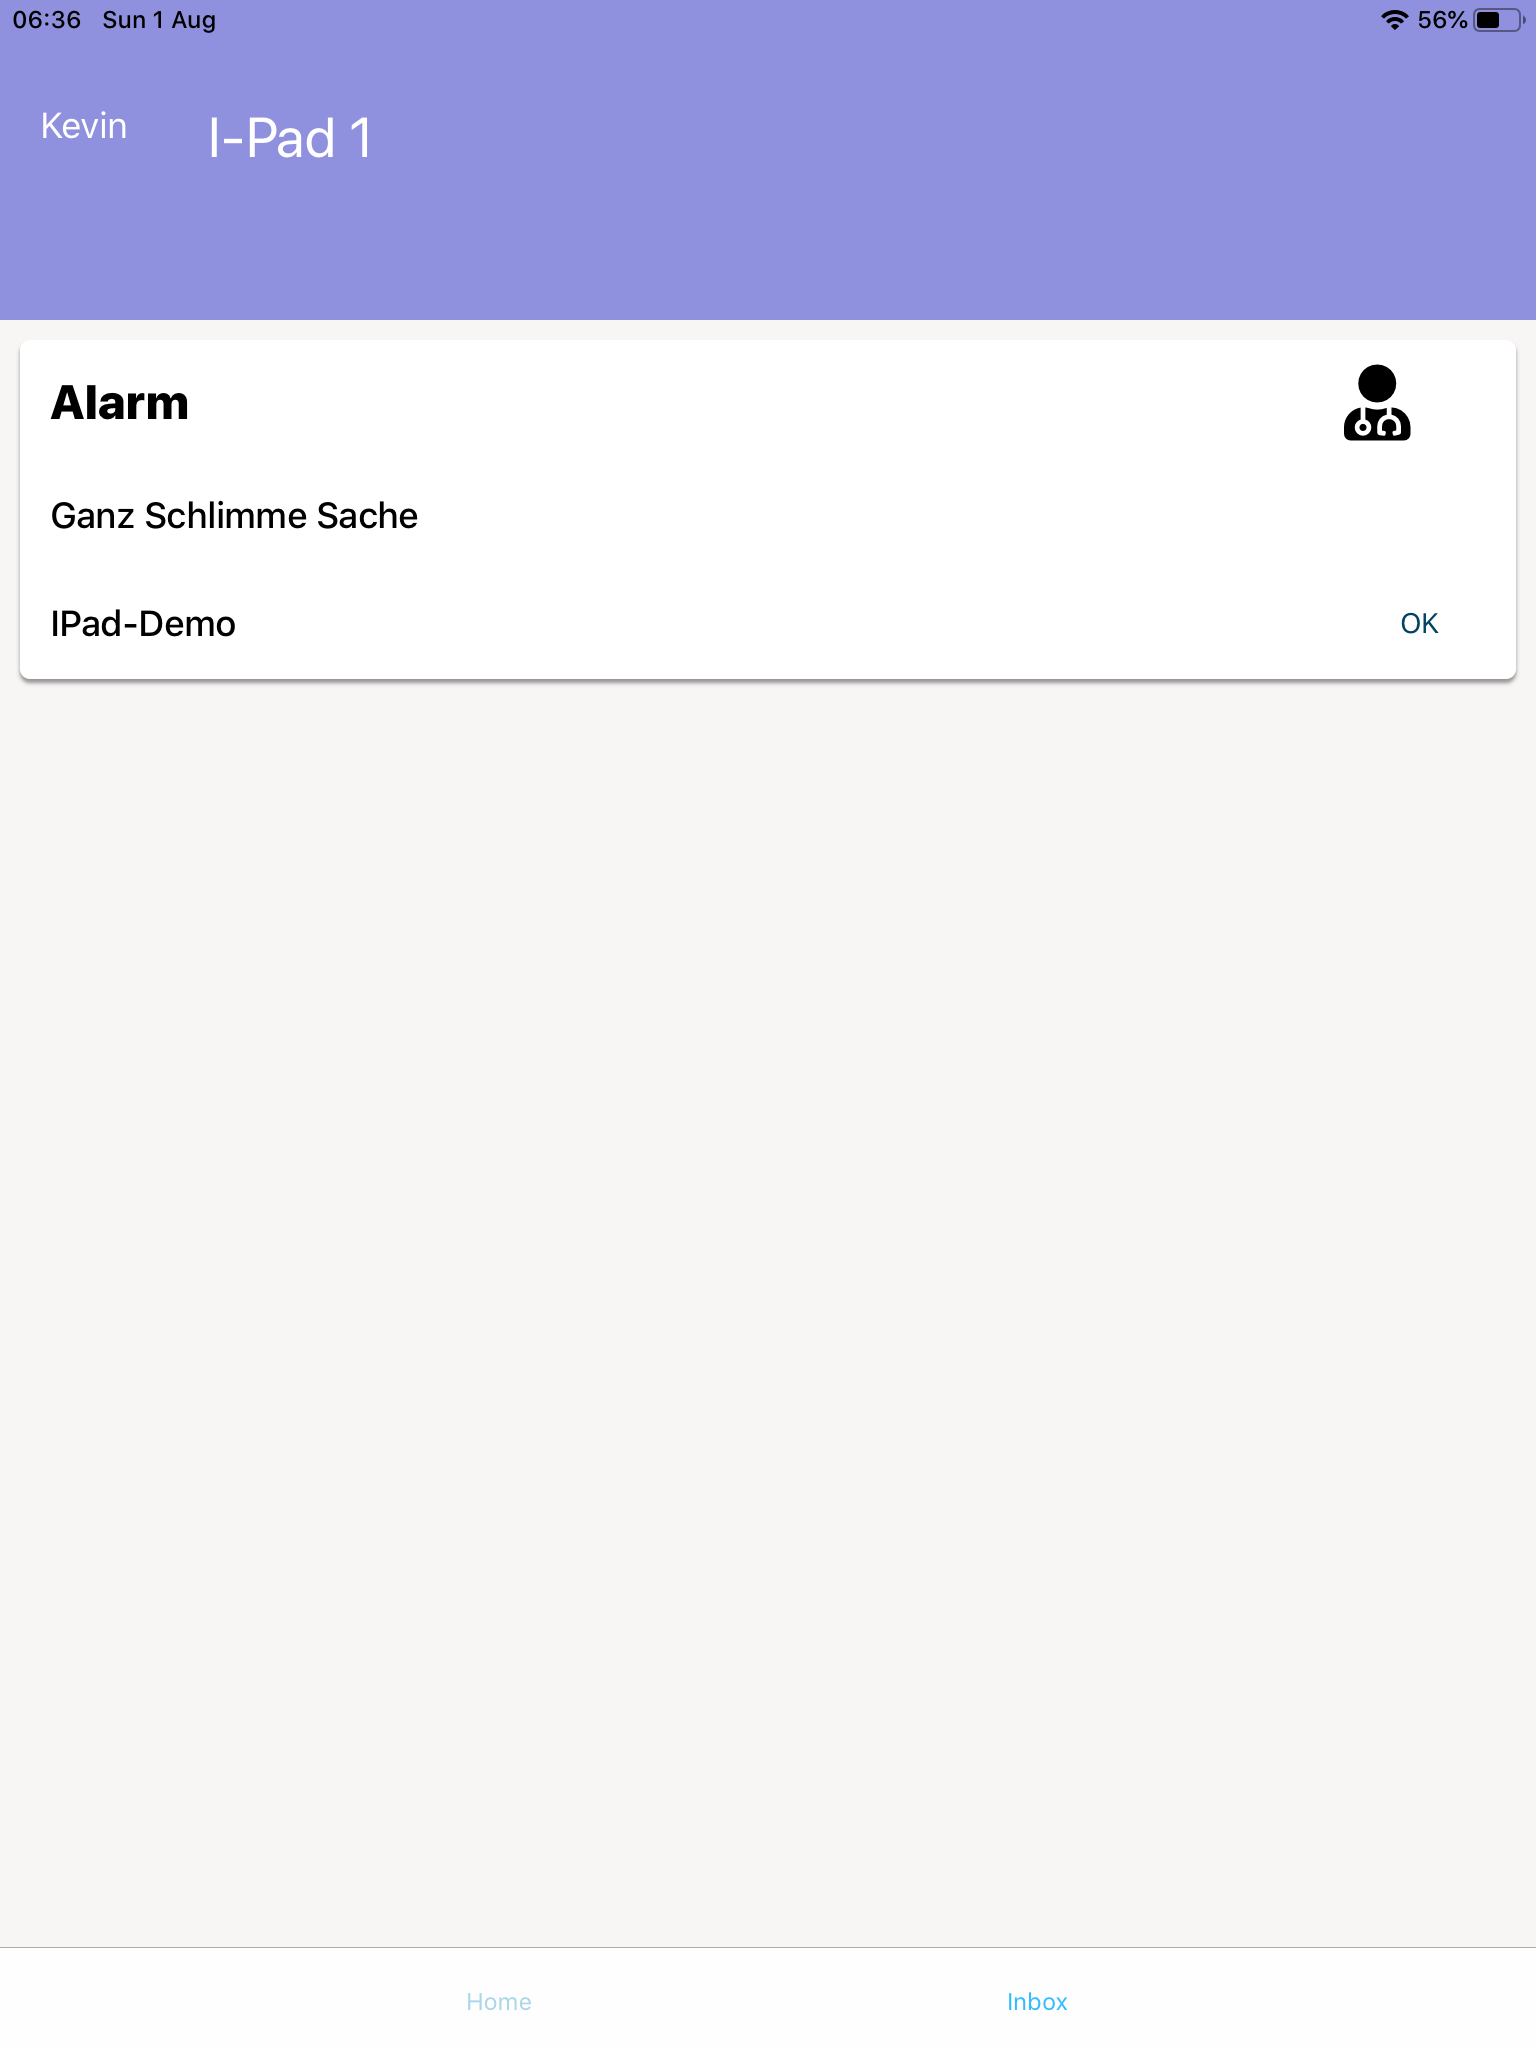
\includegraphics[width=\textwidth]{graphics/screenshots/mobileclient/screenshots-inbox}
        \caption{Inbox}
    \end{minipage}
    \label{fig:MobileClient-Screens2}
\end{figure}

\clearpage

\subsubsection{Cloud Service}

Der Cloud Service wurde wie im Konzept beschrieben umgesetzt und an den Messaging Service angebunden.

Die API ist unter www.praxisruf.ch/api erreichbar.
www.praxisruf.ch/swagger-ui.html bietet zudem zu Testzwecken die Möglichkei die Endpoints direkt anzusprechen.

\begin{minipage}[b]{1\textwidth}
    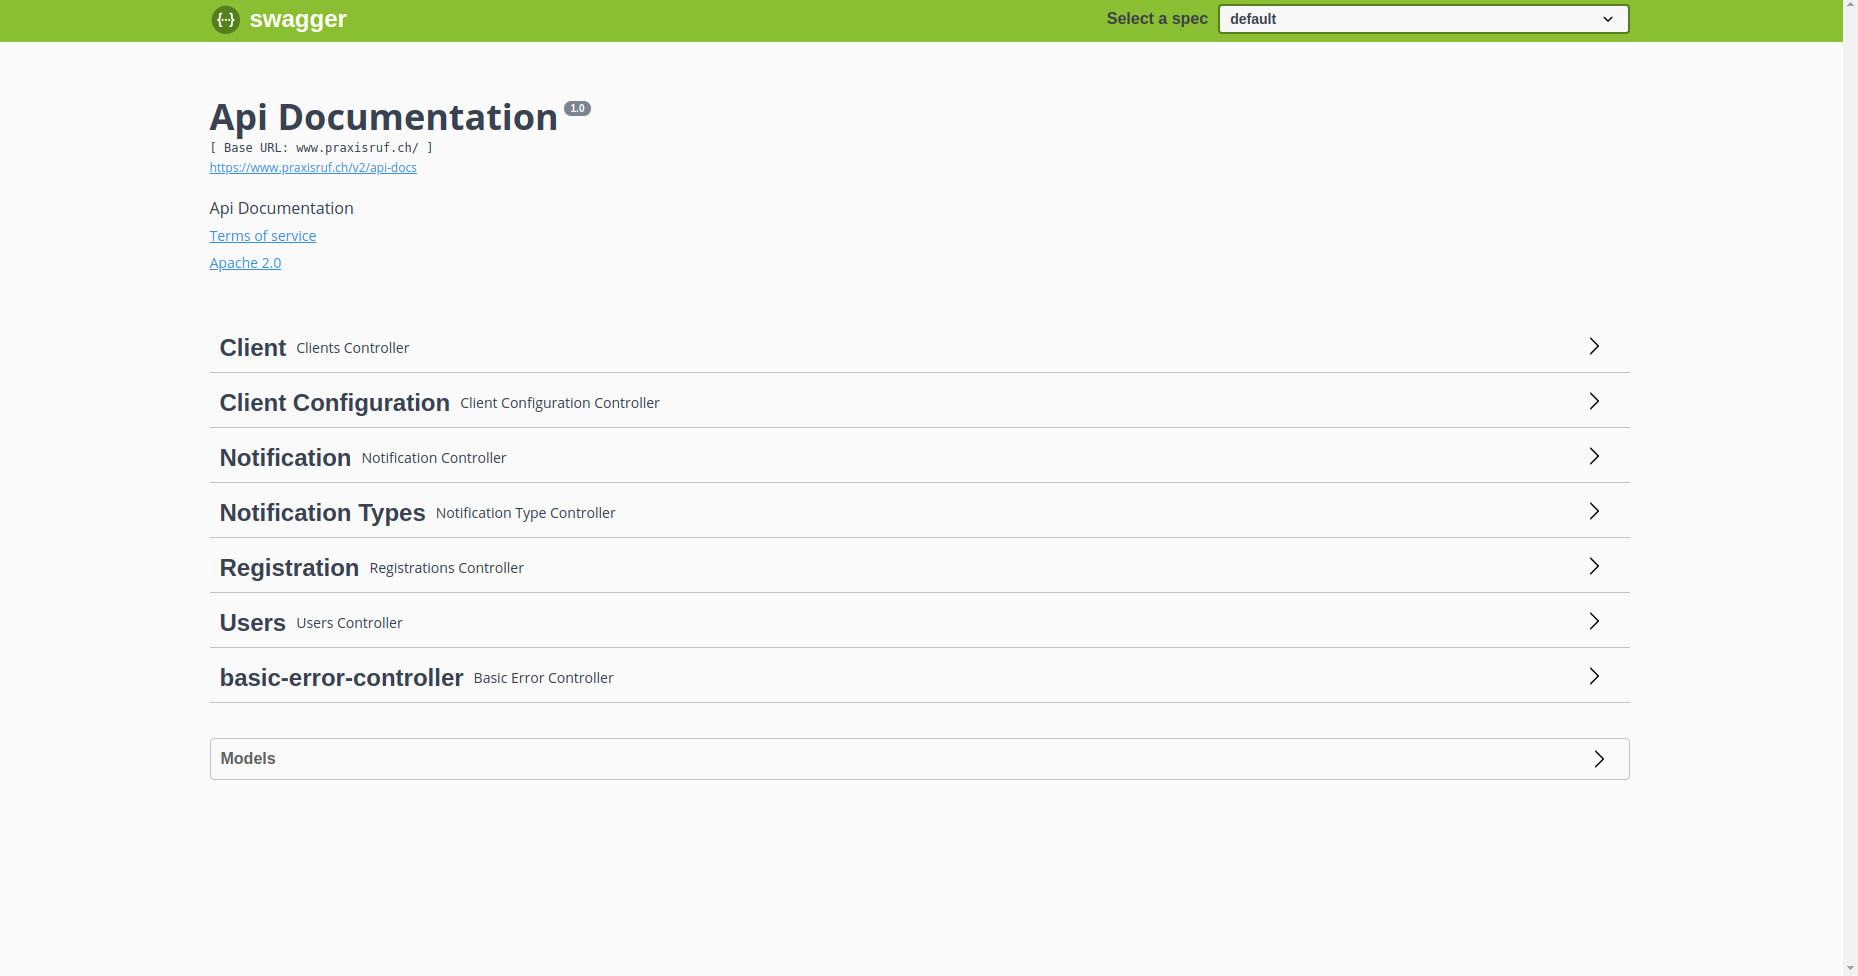
\includegraphics[width=\textwidth]{graphics/screenshots/cloud/swagger-home}
    \caption{Home}
\end{minipage}

Sorgt neben der API auch die Authentifikation die umgesetzt wurde.

\clearpage

\subsubsection{Admin UI}

\begin{figure}[h]
    \centering
    \begin{minipage}[b]{0.4\textwidth}
        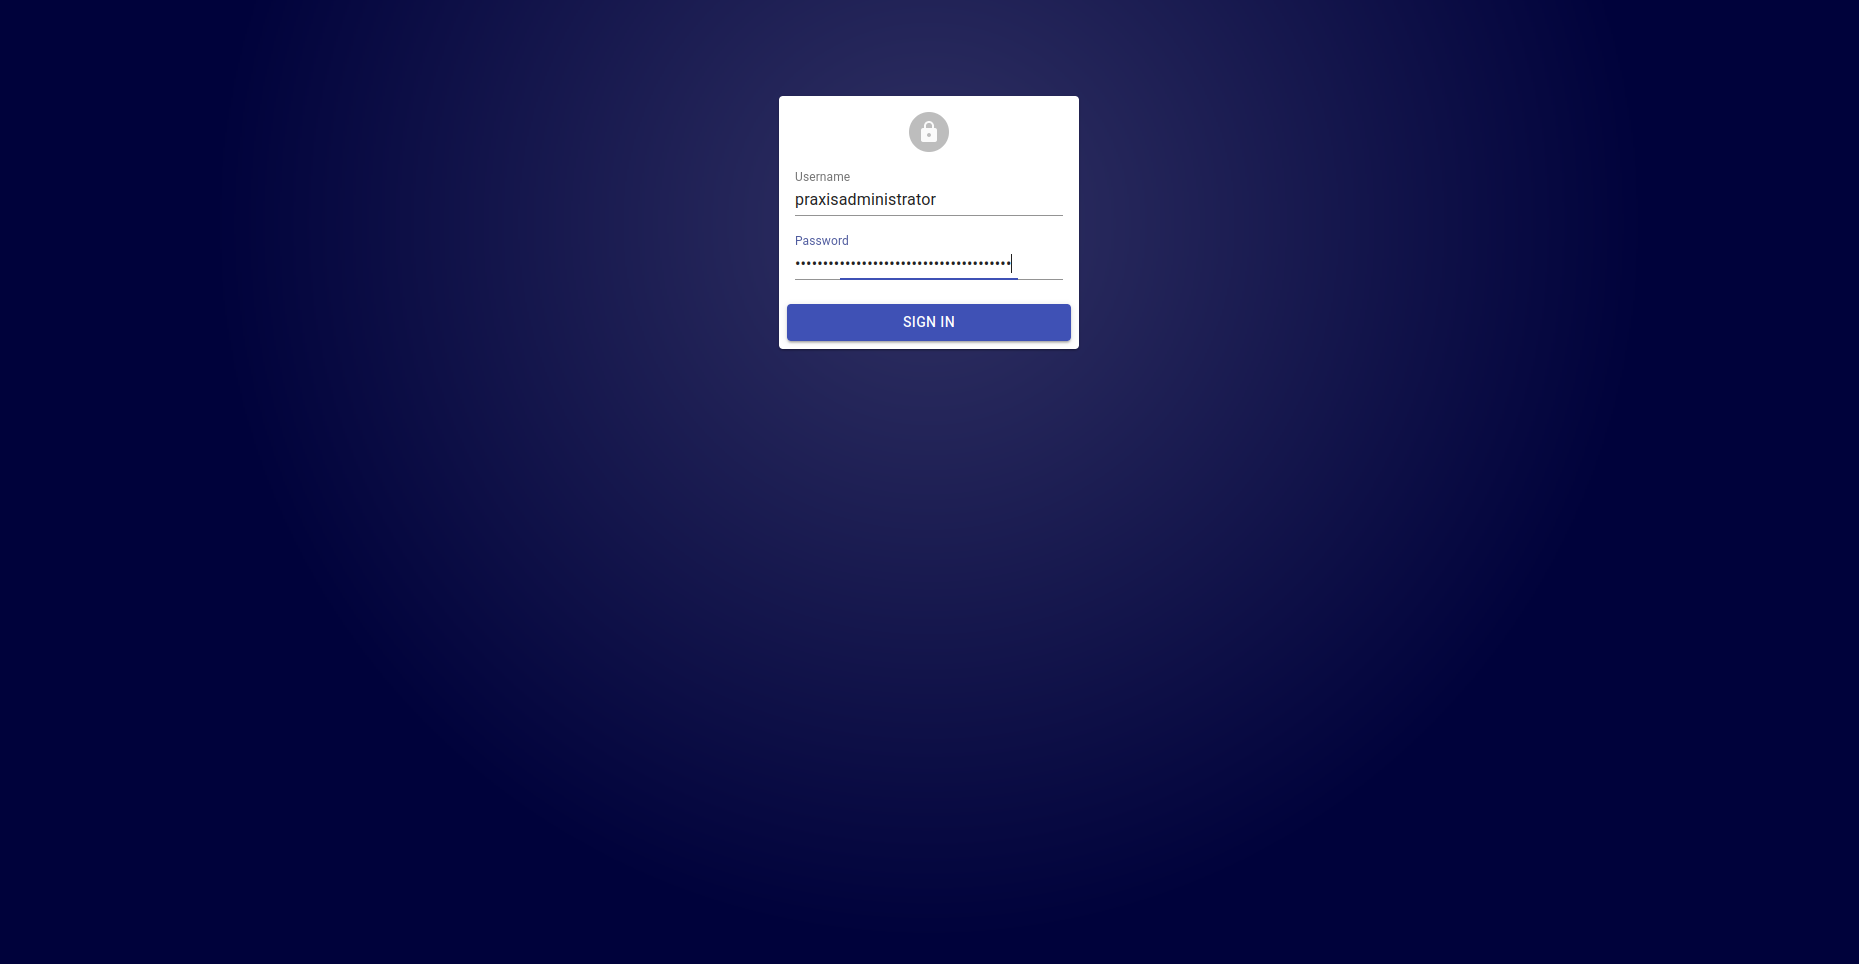
\includegraphics[width=\textwidth]{graphics/screenshots/adminui/login}
        \caption{Login}
    \end{minipage}
    \hfill
    \begin{minipage}[b]{0.4\textwidth}
        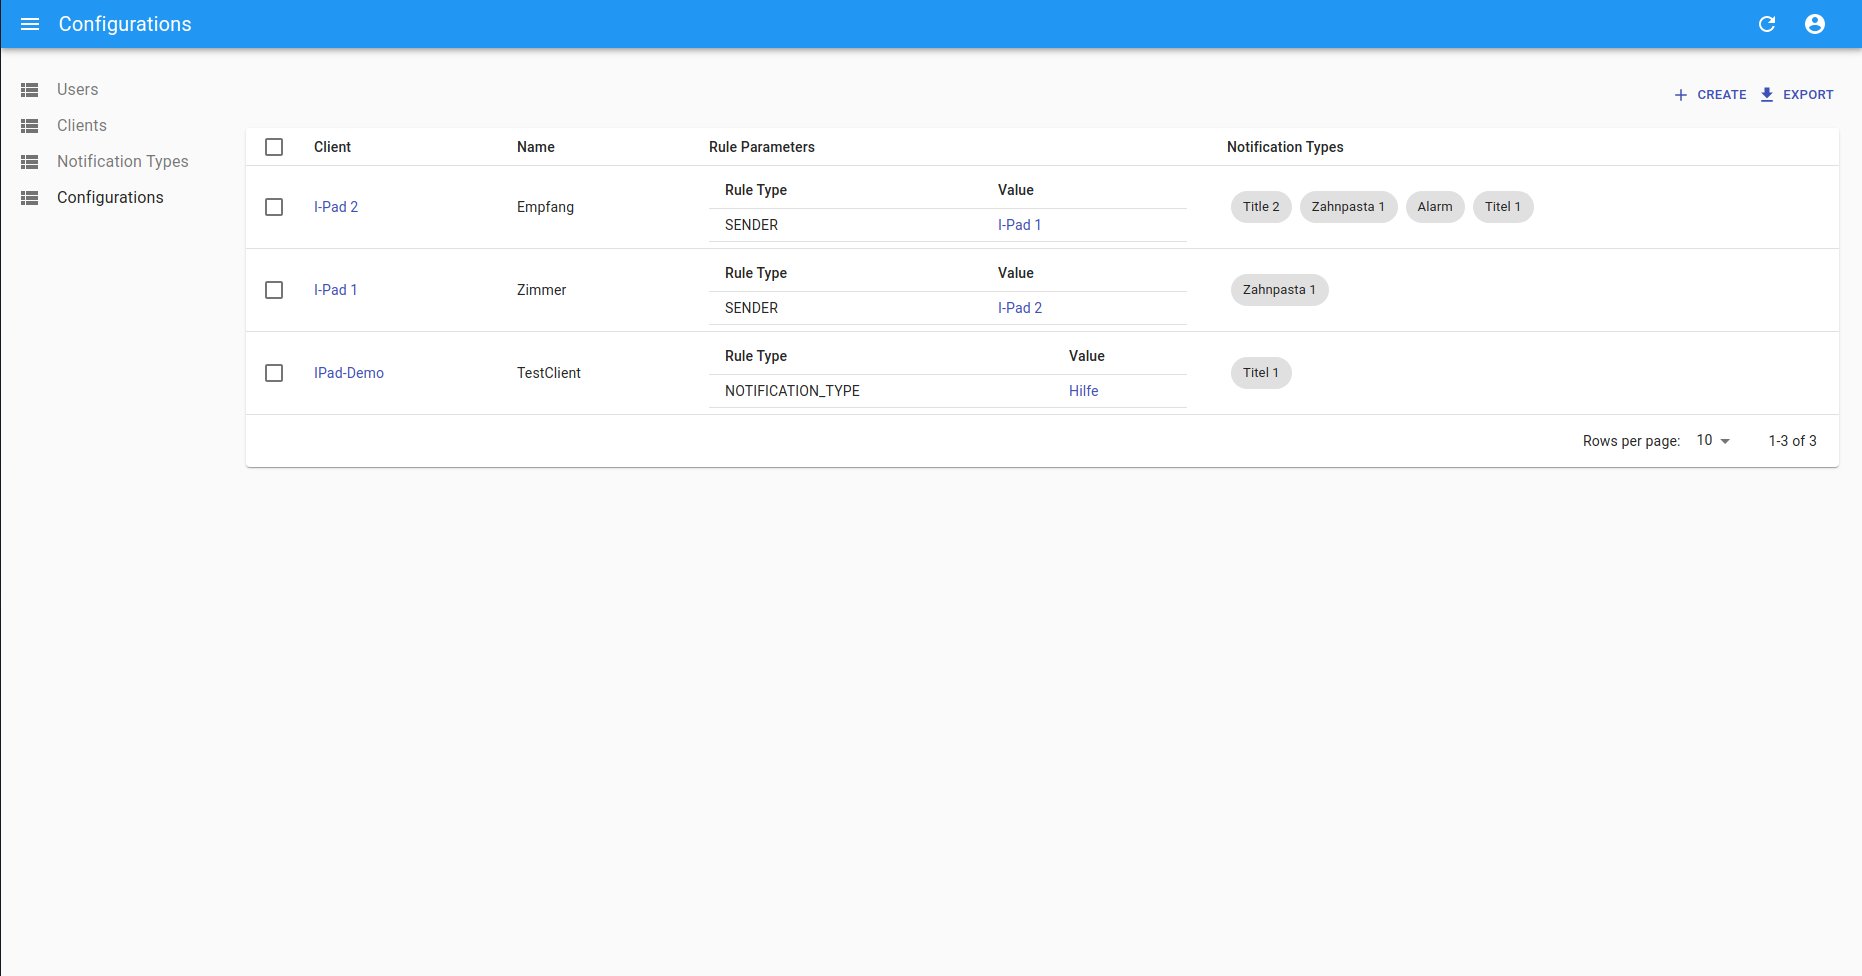
\includegraphics[width=\textwidth]{graphics/screenshots/adminui/configuration-all}
        \caption{Configuration Overview}
    \end{minipage}
    \label{fig:AdminUI-Screens1}
\end{figure}

\begin{figure}[h]
    \centering
    \begin{minipage}[b]{0.4\textwidth}
        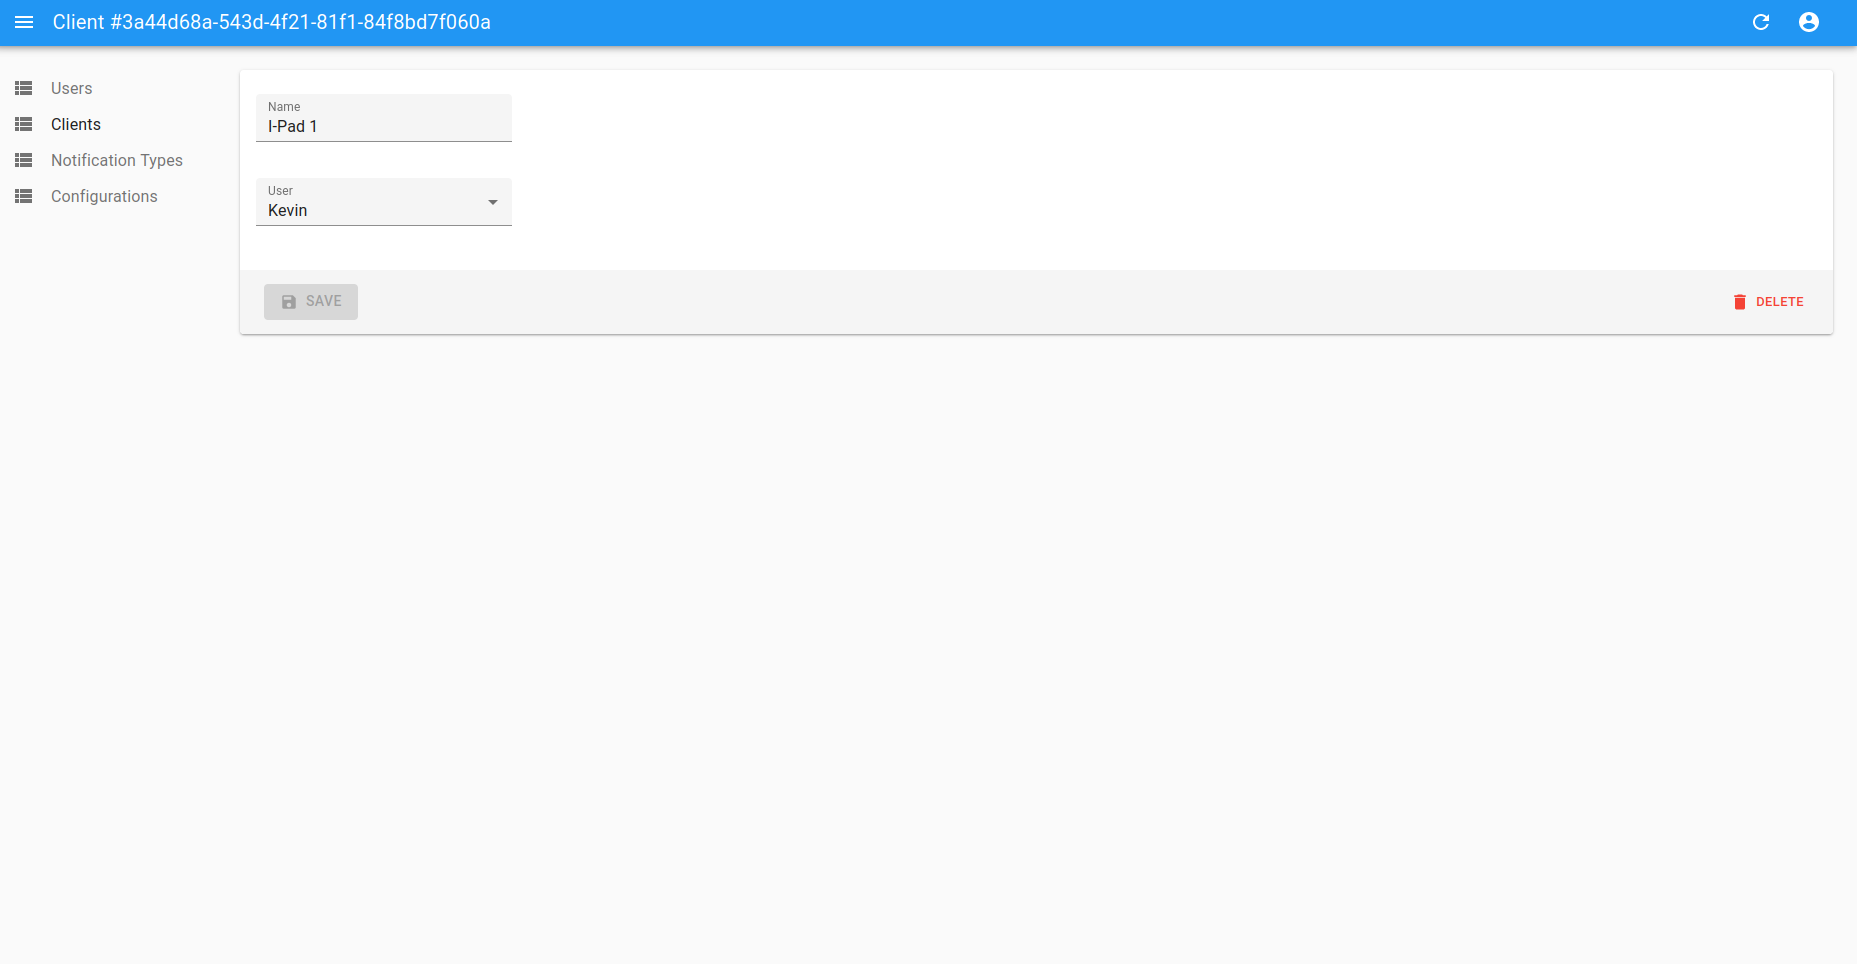
\includegraphics[width=\textwidth]{graphics/screenshots/adminui/configuration}
        \caption{Login}
    \end{minipage}
    \hfill
    \begin{minipage}[b]{0.4\textwidth}
        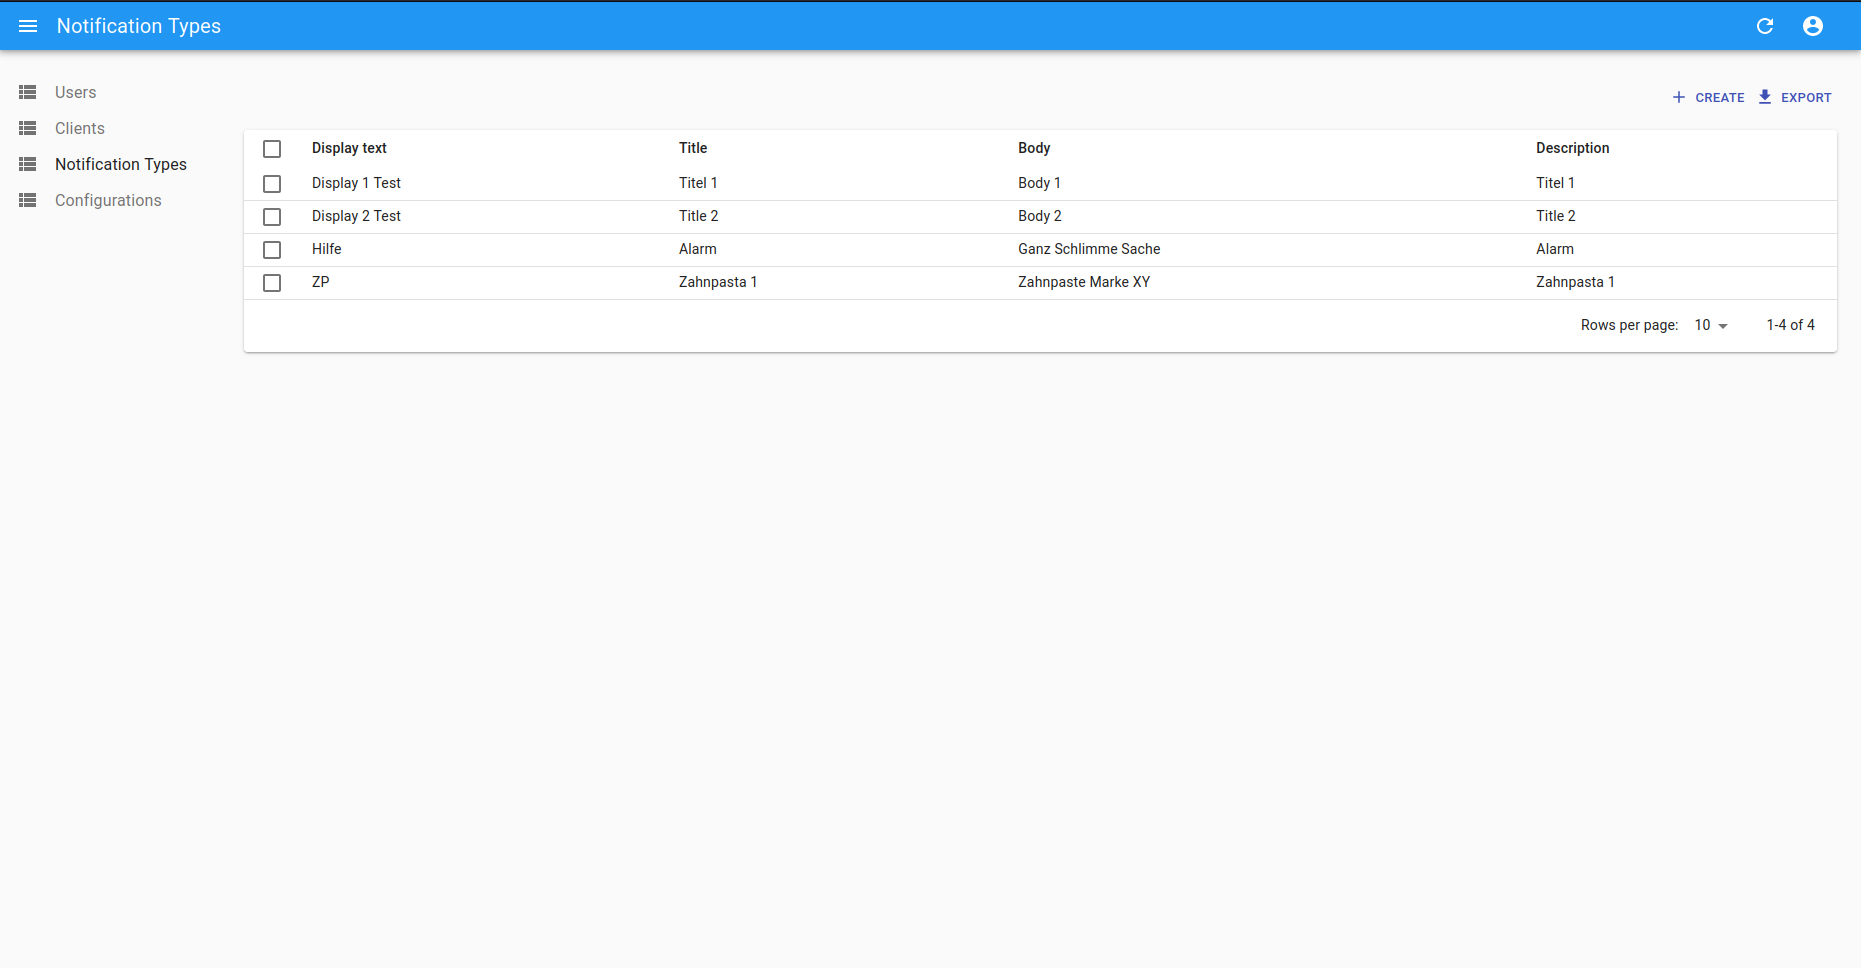
\includegraphics[width=\textwidth]{graphics/screenshots/adminui/notification-type}
        \caption{Configuration Overview}
    \end{minipage}
    \label{fig:AdminUI-Screens2}
\end{figure}




Add some screen shots

\subsection{Tests}

\subsubsection*{Benutzertests}
Wurden mit Daniel Jossen zusannem an der FH gemacht.
Mehr Tests waren wegen Ferienabwesenheiten auf Kundenseite nicht möglich.
Macht nicht so viel sinn mit nur einem Ipad.


\subsubsection*{Benutzertests}
Macht nicht so viel sinn mit nur einem Ipad.

\clearpage
\subsection{Lessons Learned}

Hearusforderungen waren:
\begin{itemize}
    \item Dokumentation fehlt komplett in der Planung
    \item IOS Recherche viel aufwändiger als erwartet.
    \item Nativescript aufwändiger zu gebrauchen als erwartet.
    \item AWS aufsetzen ist alles andere als trivial
    \item Keine Erfahrung mit Mobile Development
    \item Stärkerer Roter Faden von Anfang an hätte geholfen
    \item Mehr testing, viel Mehr Testing.
    \item Refactoring kostet Zeit, kanns aber wert sein.
\end{itemize}

Darus mitgenommen haben wir:
\begin{itemize}
    \item Gute Planung macht sich bezahlt. (Roter Faden, Doku mit einplanen, Standortbestimmung)
    \item Gute Konzepte machen sich bezahlt.
    \item Best Practices gibt es aus einem Grund. (Nativ ist besser)
    \item DevOps ist schwer.
\end{itemize}






    \section {Schluss}


%%---APPENDIX----------------------------------------------------------------------------
    \begin{appendix} %Anhang
\section{Ein Anhang}

\lipsum[61-64]

%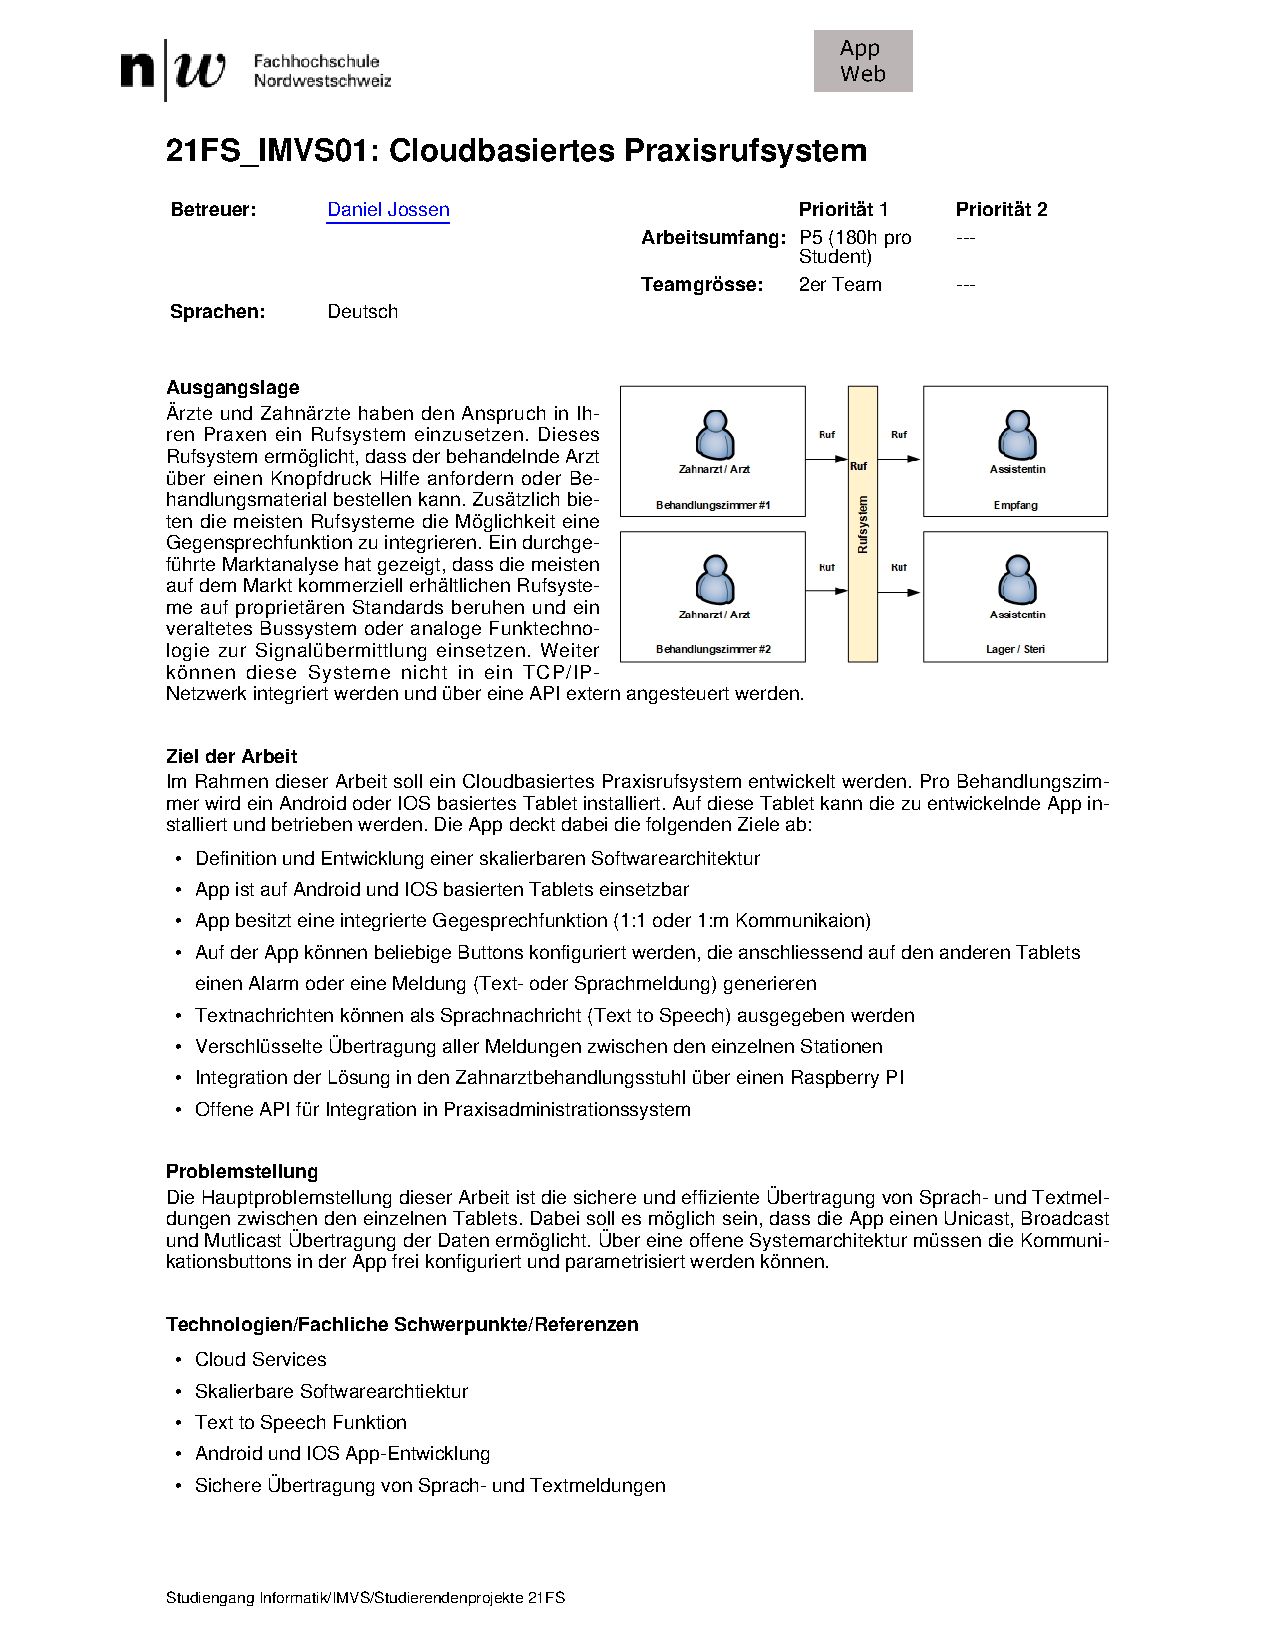
\includepdf[pages={1-2},nup=1x2,landscape=true,scale=0.85,offset=10 -40,pagecommand={\section{Eingefügtes Dokument; zwei Seiten auf einer}\label{app:Aufgabenstellung}\thispagestyle{myheadings}}]{appendix/aufgabenstellung.pdf} \newpage

%%Bei mehrseitigen Dokumenten die folgenden Seiten ohne Überschrift:
%\includepdf[pages={3-6},nup=1x2,landscape=true,scale=0.85,offset=10 -40,pagecommand={\thispagestyle{myheadings}}]{appendix/aufgabenstellung.pdf} \newpage

%\includepdf[pages={1},nup=1x1,landscape=true,scale=0.85,offset=10 -40,pagecommand={\section{Eingefügte PDF-Tabelle}\label{app:Timetable}\thispagestyle{myheadings}}]{appendix/timeline_example.pdf} \newpage

%%Bei mehrseitigen Dokumenten die folgenden Seiten ohne Überschrift:
%\includepdf[pages={2-5},nup=1x1,landscape=true,scale=0.85,offset=0 -20,pagecommand={\thispagestyle{myheadings}}]{appendix/timeline_example.pdf} \newpage

\end{appendix}


\end{document}
